\documentclass[tikz,border=2pt]{standalone}
\usepackage{amsmath}
\begin{document}
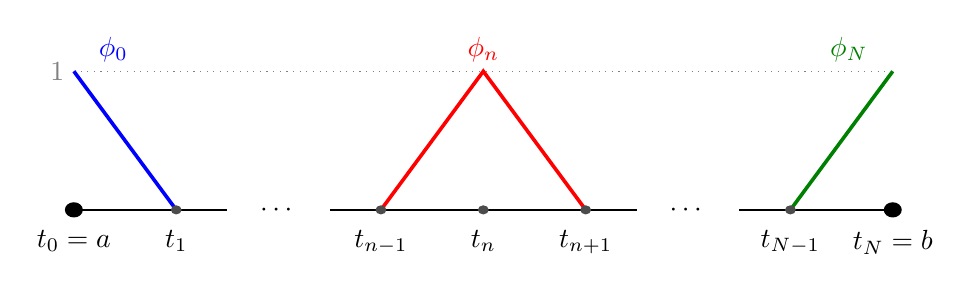
\begin{tikzpicture}[xscale=1.3, yscale=1.1,
    hat/.style={line width=1.3pt},
    ]
    \def\h{1.6} % height of the hats
    % grid line with gaps for the ellipses
    \draw[thick] (0,0) -- (1.5,0);
    \draw[thick] (2.5,0) -- (5.5,0);
    \draw[thick] (6.5,0) -- (8,0);
    \node at (2,0) {$\cdots$};
    \node at (6,0) {$\cdots$};
    % guide line at height 1
    \draw[dotted, gray] (0,\h) -- (8,\h);
    \node[left, gray] at (0,\h) {$1$};
    % hat functions
    \draw[hat, blue]            (0,\h) -- (1,0);
    \draw[hat, red]             (3,0) -- (4,\h) -- (5,0);
    \draw[hat, green!50!black]  (7,0) -- (8,\h);
    \node[blue, above right] at (0.15,\h) {$\phi_0$};
    \node[red, above] at (4,\h) {$\phi_n$};
    \node[green!50!black, above left] at (7.85,\h) {$\phi_N$};
    % grid points
    \foreach \x in {1,3,4,5,7} {
        \fill[gray!60!black] (\x,0) circle (1.5pt);
    }
    \fill[black] (0,0) circle (2.5pt);
    \fill[black] (8,0) circle (2.5pt);
    % labels
    \node[below=4pt] at (0,0) {$t_0 = a$};
    \node[below=4pt] at (1,0) {$t_1$};
    \node[below=4pt] at (3,0) {$t_{n-1}$};
    \node[below=4pt] at (4,0) {$t_n$};
    \node[below=4pt] at (5,0) {$t_{n+1}$};
    \node[below=4pt] at (7,0) {$t_{N-1}$};
    \node[below=4pt] at (8,0) {$t_N = b$};
\end{tikzpicture}
\end{document}
